\documentclass[11pt]{article}
\usepackage{amsmath,amsbsy,amssymb,verbatim,fullpage,ifthen,graphicx,bm,amsfonts,amsthm,url}
\usepackage{graphicx}
\usepackage{xcolor}
\newcommand{\mfile}[1]  {{\small \verbatiminput{./#1}}} % Jeff Fessler, input matlab file
\newcommand{\tmop}[1]{\ensuremath{\operatorname{#1}}}
%\newcommand*{\qed}{\hfill\ensuremath{\blacksquare}}%
\newcommand{\R}{\mathbb{R}}
\newcommand{\C}{\mathbb{C}}
\newcommand{\Z}{\mathbb{Z}}
\newcommand{\A}{\mathcal{A}}
\newcommand{\minimize}{\operatorname*{minimize\ }}
\newcommand{\maximize}{\operatorname*{maximize}}
\newcommand{\opdet}[1]{\operatorname{\textbf{det}}\left(#1\right)}
\newcommand{\optr}[1]{\operatorname{\textbf{tr}}\left(#1\right)}
%\newcommand{\AnswerDefine}{}
\newcommand{\answer}[2][blue]{\ifdefined\AnswerDefine{\color{#1}\it#2}\fi}
\newcommand{\mtx}[1]{\mathbf{#1}}
\newcommand{\vct}[1]{\mathbf{#1}}
\def \lg       {\langle}
\def \rg       {\rangle}
\def \mA {\mtx{A}}
\def \mF {\mtx{F}}
\def \mG {\mtx{G}}
\def \mI {\mtx{I}}
\def \mJ {\mtx{J}}
\def \mU {\mtx{U}}
\def \mS {\mtx{S}}
\def \mV {\mtx{V}}
\def \mW {\mtx{W}}
\def \mLambda {\mtx{\Lambda}}
\def \mSigma {\mtx{\Sigma}}
\def \mX {\mtx{X}}
\def \mY {\mtx{Y}}
\def \mZ {\mtx{Z}}
\def \zero     {\mathbf{0}}
\def \vzero    {\vct{0}}
\def \vone    {\vct{1}}
\def \va {\vct{a}}
\def \vg {\vct{g}}
\def \vu {\vct{u}}
\def \vv {\vct{v}}
\def \vx {\vct{x}}
\def \vy {\vct{y}}
\def \vz {\vct{z}}
\def \vphi {\vct{\phi}}
\def \vmu {\vct{\mu}}
\def \R {\mathbb{R}}

%\newcommand{\st}{\operatorname*{\ subject\ to\ }}
\usepackage{algorithm,algpseudocode}
\usepackage{xspace}
% Add a period to the end of an abbreviation unless there's one
% already, then \xspace.
\makeatletter
\DeclareRobustCommand\onedot{\futurelet\@let@token\@onedot}
\def\@onedot{\ifx\@let@token.\else.\null\fi\xspace}

\def\eg{\emph{e.g}\onedot} \def\Eg{\emph{E.g}\onedot}
\def\ie{\emph{i.e}\onedot} \def\Ie{\emph{I.e}\onedot}
\def\cf{\emph{c.f}\onedot} \def\Cf{\emph{C.f}\onedot}
\def\etc{\emph{etc}\onedot} \def\vs{\emph{vs}\onedot}
\def\wrt{w.r.t\onedot} \def\dof{d.o.f\onedot}
\def\etal{\emph{et al}\onedot} \def\st{\emph{s.t}\onedot}
\pagestyle{plain}

\title{{\bf Homework Set 6, CPSC 8420, Fall 2024}} % Change to the appropriate homework number
\author{\Large\underline{Last Name, First Name}}
\date{\textbf{\Large\textcolor{red}{Due 12/05/2024, 11:59PM EST}}} % put your name in the LastName, FirstName format
%\date{\today}

\begin{document}
\maketitle


\section*{Problem 1}
Frequently, the affinity matrix is constructed as:
\begin{equation}
	A_{ij}=e^{-d(x_i,x_j)^2/\sigma}
\end{equation}
where $\sigma$  is some user-specified parameter. The best that we can hope for in practice is a near block-diagonal
affinity matrix. It can be shown in this case, that after projecting to the space spanned by the top $k$
eigenvectors, points which belong to the same block are close to each other in a euclidean sense. The steps are as follows:
\begin{itemize}
	\item Construct an affinity matrix $A$ using the above equation.
	\item Symmetrically `normalize’ the rows and columns of $A$ to get a matrix $N$ such that $N(i,j)=\frac{A(i,j)}{\sqrt{d(i)d(j)}}$, where $d(i)=\sum_k A(i,k)$.
	\item Construct a matrix $Y$ whose columns are the first $k$ eigenvectors of $N$.
	\item Normalize each row of $Y$ such that it is of unit length.
	\item Cluster the dataset by running $k$-means on the set of  embedded points, where each row of $Y$ is a data-point.
\end{itemize}

\begin{enumerate}
	\item Run $k$-means on the datasets provided in the .zip file. For text.mat, take $k = 6$. For all others use $k = 2$.
	\item  Implement the above spectral clustering algorithm and run it on the four provided datasets using the same $k$. Plot your clustering results using $\sigma = .025, .05, .2, .5$. Hints: You may find the MATLAB functions pdist and eig to be helpful. A function plotClusters.m has been provided to help visualize clustering results.
	\item Plot the first 10 eigenvalues for the rectangles.mat and text.mat datasets when $\sigma = .05$. What do you notice?
	\item How do $k$-means and spectral clustering compare?
\end{enumerate}
\begin{figure}[h!]
	\centering
	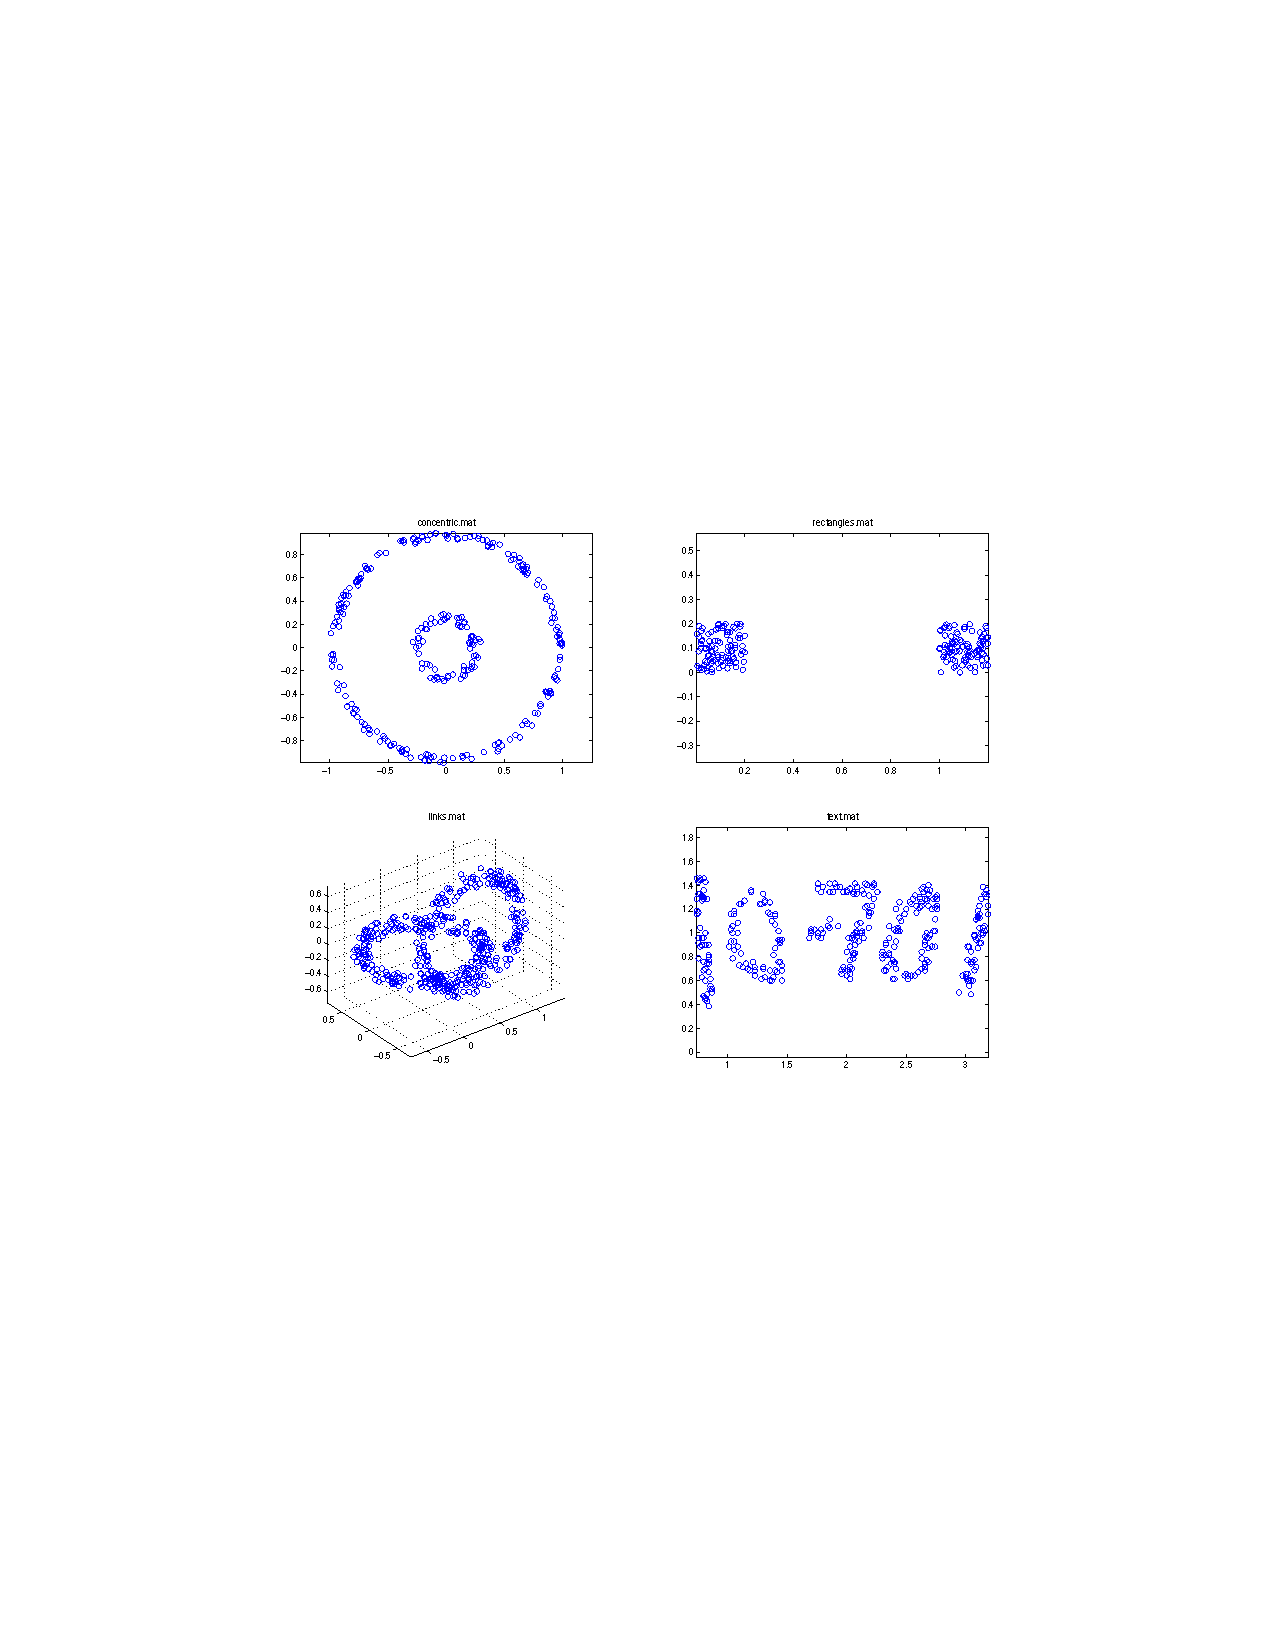
\includegraphics[width=\linewidth]{syn}
\end{figure}
\end{document}
